\documentclass{beamer}

\mode<presentation>
\usepackage{amsmath,amssymb,mathtools}
\usepackage{textcomp}
\usepackage{gensymb}
\usepackage{adjustbox}
\usepackage{subcaption}
\usepackage{enumitem}
\usepackage[utf8]{inputenc}
\usepackage{amssymb}
\usepackage{newunicodechar}
\usepackage{enumitem}
\setlist{nosep} % optional: removes vertical gaps
\setlist[enumerate]{label=\arabic*)} % custom numbering if you want

\newunicodechar{√}{$\sqrt{\;}$}
\newunicodechar{✅}{\checkmark}
\newunicodechar{❌}{\texttimes}
\usepackage{multicol}
\usepackage{listings}
\usepackage{url}
\usepackage{graphicx} % <-- needed for images
\def\UrlBreaks{\do\/\do-}

\usetheme{Boadilla}
\usecolortheme{lily}
\setbeamertemplate{footline}{
  \leavevmode%
  \hbox{%
  \begin{beamercolorbox}[wd=\paperwidth,ht=2ex,dp=1ex,right]{author in head/foot}%
    \insertframenumber{} / \inserttotalframenumber\hspace*{2ex}
  \end{beamercolorbox}}%
  \vskip0pt%
}
\setbeamertemplate{navigation symbols}{}

\lstset{
  frame=single,
  breaklines=true,
  columns=fullflexible,
  basicstyle=\ttfamily\tiny   % tiny font so code fits
}

\numberwithin{equation}{section}

% ---- your macros ----
\providecommand{\nCr}[2]{\,^{#1}{#2}}
\providecommand{\nPr}[2]{\,^{#1}P_{#2}}
\providecommand{\mbf}{\mathbf}
\providecommand{\pr}[1]{\ensuremath{\Pr\left(#1\right)}}
\providecommand{\qfunc}[1]{\ensuremath{Q\left(#1\right)}}
\providecommand{\sbrak}[1]{\ensuremath{{}\left[#1\right]}}
\providecommand{\lsbrak}[1]{\ensuremath{{}\left[#1\right.}}
\providecommand{\rsbrak}[1]{\ensuremath{\left.#1\right]}}
\providecommand{\brak}[1]{\ensuremath{\left(#1\right)}}
\providecommand{\lbrak}[1]{\ensuremath{\left(#1\right.}}
\providecommand{\rbrak}[1]{\ensuremath{\left.#1\right)}}
\providecommand{\cbrak}[1]{\ensuremath{\left\{#1\right\}}}
\providecommand{\lcbrak}[1]{\ensuremath{\left\{#1\right.}}
\providecommand{\rcbrak}[1]{\ensuremath{\left.#1\right\}}}
\theoremstyle{remark}
\newtheorem{rem}{Remark}
\newcommand{\sgn}{\mathop{\mathrm{sgn}}}
\providecommand{\abs}[1]{\left\vert#1\right\vert}
\providecommand{\res}[1]{\Res\displaylimits_{#1}}
\providecommand{\norm}[1]{\lVert#1\rVert}
\providecommand{\mtx}[1]{\mathbf{#1}}
\providecommand{\mean}[1]{E\left[ #1 \right]}
\providecommand{\fourier}{\overset{\mathcal{F}}{ \rightleftharpoons}}
\providecommand{\system}{\overset{\mathcal{H}}{ \longleftrightarrow}}
\providecommand{\dec}[2]{\ensuremath{\overset{#1}{\underset{#2}{\gtrless}}}}
\newcommand{\myvec}[1]{\ensuremath{\begin{pmatrix}#1\end{pmatrix}}}
\let\vec\mathbf
% ---------------------

\title{Matgeo Presentation - Problem 4.13.26}
\author{ee25btech11021 - Dhanush sagar}

\begin{document}
	

		




%---------------- Title Page ----------------
\begin{frame}
  \titlepage
\end{frame}

%---------------- Problem Statement ----------------
\begin{frame}{Problem Statement}
A straight the through a fixed point (2, 3) intersects the coordinate axes at distinct
points P and Q. If O is the origin and the rectangle OPRQ is completed, then the
locus of R is 
\end{frame}

%---------------- Mathematical Formula ----------------
\begin{frame}{solution}

% --- Step 1: Equation of line through fixed point ---
\text{Equation of a line with normal vector $\vec{n}$ through } \myvec{2\\3}:
\begin{align}
\vec{n}^T\vec{x} &= \vec{n}^T\myvec{2\\3}  
\end{align}

% --- Step 2: Intercepts with axes ---
\text{The $x$-intercept is} $\vec{P}=\myvec{p\\0}$.
\text{The $y$-intercept is} $\vec{Q}=\myvec{0\\q}$. \\



% --- Step 3: Vertices of the rectangle ---
\text{The origin is}
\begin{align}
\vec{O} &= \myvec{0\\0}  
\end{align}




% --- Step 2: Relate u to the intercepts P and Q ---

\text{If the intercepts are } $\vec{P}=\myvec{p\\0},\; \vec{Q}=\myvec{0\\q}$, \text{ then normal vector is } 
\begin{align}
\vec{n} &= \myvec{\tfrac{1}{p}\\[3pt]\tfrac{1}{q}}
\end{align}
\end{frame}
\begin{frame}{solution}
% --- Step 3: Opposite vertex R of rectangle OPRQ ---
\text{The opposite vertex of rectangle OPRQ is then } 
\begin{align}
\vec{R} &= \myvec{p\\[3pt]q}
\end{align}

% --- Step 4: Express the condition u^T(2,3)=1 in terms of R ---
\text{Write } $\vec{n}$ \text{ in terms of } $\vec{R}$ \text{ by }
\begin{align}
\vec{n}=\myvec{\tfrac{1}{p}\\[3pt]\tfrac{1}{q}}=\myvec{\tfrac{1}{x}\\[3pt]\tfrac{1}{y}}\text{ where } \vec{R}=\myvec{x\\y}:
\end{align}
\begin{align}
\myvec{\tfrac{1}{x} & \tfrac{1}{y}}\myvec{2\\3} &= 1
\end{align}


% --- Step 5: Multiply out and clear denominators to obtain locus ---
\text{Multiply out the left-hand side:}
\begin{align}
\tfrac{2}{x} + \tfrac{3}{y} &= 1
\end{align}

\text{Clear denominators by multiplying both sides by } xy:
\begin{align}
2y + 3x &= xy
\end{align}
\end{frame}
\begin{frame}{solution}
\text{Rearrange to standard quadratic form:}
\begin{align}
xy - 3x - 2y &= 0
\end{align}

% --- Step 7: Expressing in quadratic form ---
\text{A conic in matrix form is } 
\begin{align}
\vec{x}^T \vec{V} \vec{x} + 2 \vec{u}^T \vec{x} + f = 0, \quad \vec{x} = \myvec{x\\y}.
\end{align}



\text{Here, the matrix corresponding to the } xy \text{ term is symmetric:}
\begin{align}
\vec{V} &= \myvec{0 & \tfrac{1}{2} \\[1mm] \tfrac{1}{2} & 0}, \quad
\vec{u} = \myvec{-3\\-2}, \quad f = 0
\end{align}

% --- Step 7: Final locus in matrix form ---
\begin{align}
\vec{x}^T \myvec{0 & \tfrac{1}{2} \\[1mm] \tfrac{1}{2} & 0} \vec{x} + 2 \myvec{-3\\-2}^T \vec{x} &= 0
\end{align}

\end{frame}
%---------------- C Source Code ----------------
\begin{frame}[fragile]{C Source Code:nor line.c}
\begin{verbatim}
#include <stdio.h>
#include <stdlib.h>

// Line passing through (2,3) with slope m
void generate_line_points(double m, double* P, double* Q) {
    // X-intercept (y=0)
    double x_intercept = 2.0 - 3.0 / m;
    // Y-intercept (x=0)
    double y_intercept = 3.0 - 2.0 * m;

    P[0] = x_intercept; P[1] = 0.0;
    Q[0] = 0.0; Q[1] = y_intercept;
}



\end{verbatim}
\end{frame}

%---------------- Python solve.py ----------------
\begin{frame}[fragile]{Python Script:solve-r.py}
\begin{verbatim}
import ctypes
import numpy as np

# Load C library
lib = ctypes.CDLL("./nor_points.so")
lib.generate_line_points.argtypes = [
    ctypes.c_double,
    ctypes.POINTER(ctypes.c_double),
    ctypes.POINTER(ctypes.c_double)
]

def get_line_points(m):
    P = (ctypes.c_double * 2)()
    Q = (ctypes.c_double * 2)()
    lib.generate_line_points(ctypes.c_double(m), P, Q)
    return np.array([P[0], P[1]]), np.array([Q[0], Q[1]])



\end{verbatim}
\end{frame}
\begin{frame}[fragile]{Python Script:solve-r.py}
\begin{verbatim}
def compute_R_points(m_values):
    R_points = []
    for m in m_values:
        if m == 0:  # avoid horizontal line
            continue
        P, Q = get_line_points(m)
        R = P + Q
        R_points.append(R)
    return np.array(R_points)

if __name__ == "__main__":
    # Use fine slope sampling for smooth curve
    slopes = np.linspace(-50, 50, 2000)
    R_pts = compute_R_points(slopes)
    np.save("R_points.npy", R_pts)

\end{verbatim}
\end{frame}

\begin{frame}[fragile]{Python Script: plot-r.py}
\begin{verbatim}
import numpy as np
import matplotlib.pyplot as plt
# Load computed R points
R_points = np.load("R_points.npy")
# Remove any points with extremely large values (slope ~ 0)
mask = (np.abs(R_points[:,0]) < 1000) & (np.abs(R_points[:,1]) < 1000)
R_points = R_points[mask]
# Plot the locus of R
plt.figure(figsize=(8,6))
plt.plot(R_points[:,0], R_points[:,1], color='red', linewidth=2)
plt.title("Locus of R for rectangle OPRQ")
plt.xlabel("X-axis")
plt.ylabel("Y-axis")
plt.grid(True)
plt.axhline(0, color='black')
plt.axvline(0, color='black')
plt.show()


\end{verbatim}
\end{frame}

%---------------- Result Plot ----------------
\begin{frame}{Result Plot}
 \begin{figure}[H]
     \centering
     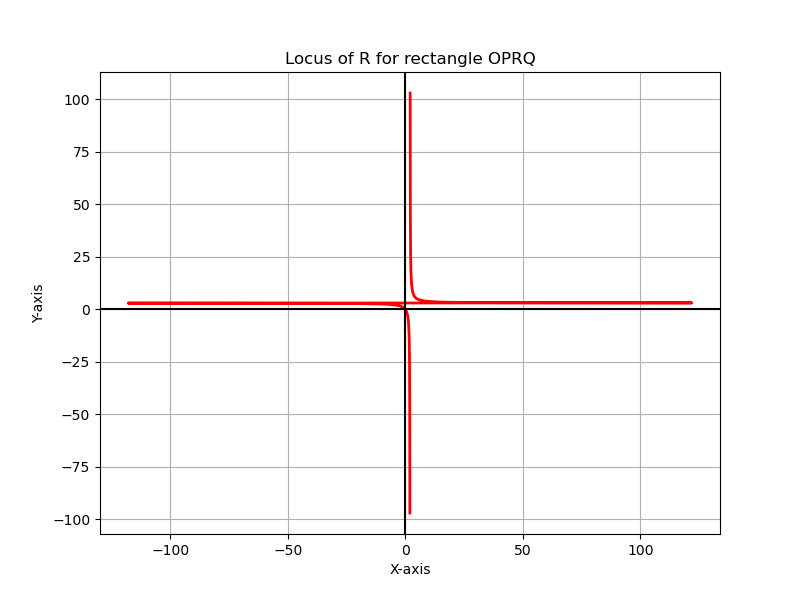
\includegraphics[width=0.7\columnwidth]{figs/fig1.png}
     \caption*{}
     \label{fig:fig1}
 \end{figure}
 
\end{frame}

\end{document}
\end{document}
